%%% Preamble
\documentclass{report}

\usepackage[utf8]{inputenc}
\usepackage[T1]{fontenc}
\usepackage{fourier}
\usepackage[french]{babel}
\usepackage[protrusion=true,expansion=true]{microtype}	
\usepackage{amsmath,amsfonts,amsthm} % Math packages
\usepackage[pdftex]{graphicx}	
\usepackage{url}
\usepackage{pdfpages}
\usepackage{todonotes}
\usepackage[a4paper, body={16cm,26cm}]{geometry}
\usepackage{float}
\usepackage{framed}
\usepackage[toc,page]{appendix} 
\usepackage{multicol}
\usepackage{colortbl}
\usepackage{epstopdf}
\usepackage{adjustbox}

%%% Custom sectioning
\usepackage{sectsty}
\allsectionsfont{  \normalfont\scshape}
%\allsectionsfont{\centering \normalfont\scshape}

%%% Custom headers/footers (fancyhdr package)
\usepackage{fancyhdr}
\pagestyle{fancyplain}
\fancyhead{}								% No page header
\fancyfoot[L]{}							% Empty 
\fancyfoot[C]{}							% Empty
\fancyfoot[R]{\thepage}					% Pagenumbering
\renewcommand{\headrulewidth}{0pt}		% Remove header underlines
\renewcommand{\footrulewidth}{0pt}		% Remove footer underlines
\setlength{\headheight}{13.6pt}


%%% Equation and float numbering
\numberwithin{equation}{section}		% Equationnumbering: section.eq#
\numberwithin{figure}{section}		% Figurenumbering: section.fig#
\numberwithin{table}{section}		% Tablenumbering: section.tab#


%%% Define new commands
\newcommand{\horrule}[1]{\rule{\linewidth}{#1}} 	% Horizontal rule
\renewcommand{\bf}[1]{\textbf{#1}}
\renewcommand{\it}[1]{\textit{#1}}
\newcommand{\bfit}[1]{\textbf{\textit{#1}}}
\renewcommand{\sc}[1]{\textsc{#1}}

\newcommand{\Todo}[1]{\todo[inline]{#1}}
\renewcommand{\thesection}{\thepart .\arabic{section}}

\usepackage{tocloft}
\cftsetindents{chapter}{0em}{1em}
\cftsetindents{section}{1.5em}{2.5em}
\makeatletter
\def\l@figure{\@dottedtocline{1}{1.5em}{4em}}
\makeatother

\usepackage{bookmark}
%\usepackage[hidelinks]{hyperref}
\usepackage{cases}
\usepackage{color}
\usepackage{xcolor}
\usepackage{relsize}
\usepackage{caption}
\colorlet{shadecolor}{black!10}

\delimitershortfall-1sp
\newcommand\abs[1]{\left|#1\right|}


\usepackage{tikz, pgfplots}


%}}}
%{{{ --- pgfplots ---------------------

%{{{ Colors

% TolColors from http://www.r-bloggers.com/the-paul-tol-21-color-salute/
\definecolor{TolColor1}{HTML}{332288}   % dark purple
\definecolor{TolColor2}{HTML}{6699CC}   % dark blue
\definecolor{TolColor3}{HTML}{88CCEE}   % light blue
\definecolor{TolColor4}{HTML}{44AA99}   % light green
\definecolor{TolColor5}{HTML}{117733}   % dark green
\definecolor{TolColor6}{HTML}{999933}   % dark brown
\definecolor{TolColor7}{HTML}{DDCC77}   % light brown
\definecolor{TolColor8}{HTML}{661100}   % dark red
\definecolor{TolColor9}{HTML}{CC6677}   % light red
\definecolor{TolColor10}{HTML}{AA4466}  % light pink
\definecolor{TolColor11}{HTML}{882255}  % dark pink
\definecolor{TolColor12}{HTML}{AA4499}  % light purple

%}}}
%{{{ Color cycles

\pgfplotscreateplotcyclelist{mbarplot cycle}{%
  {draw=TolColor2, fill=TolColor2!70},
  {draw=TolColor7, fill=TolColor7!70},
  {draw=TolColor4, fill=TolColor4!70},
  {draw=TolColor11, fill=TolColor11!70},
  {draw=TolColor1, fill=TolColor1!70},
  {draw=TolColor8, fill=TolColor8!70},
  {draw=TolColor6, fill=TolColor6!70},
  {draw=TolColor9, fill=TolColor9!70},
  {draw=TolColor10, fill=TolColor10!70},
  {draw=TolColor12, fill=TolColor12!70},
  {draw=TolColor3, fill=TolColor3!70},
  {draw=TolColor5, fill=TolColor5!70},
}

\pgfplotscreateplotcyclelist{mlineplot cycle}{%
  {TolColor2, mark=*, mark size=1.5pt},
  {TolColor7, mark=square*, mark size=1.3pt},
  {TolColor4, mark=triangle*, mark size=1.5pt},
  {TolColor6, mark=diamond*, mark size=1.5pt},
}


\pgfplotsset{
  compat=1.9,
  mbaseplot/.style={
    legend style={
      draw=none,
      fill=none,
      cells={anchor=west},
    },
    x tick label style={
      font=\footnotesize
    },
    y tick label style={
      font=\footnotesize
    },
    legend style={
      font=\footnotesize
    },
    major grid style={
      dotted,
    },
    axis x line*=bottom,
  },
  mlineplot/.style={
    mbaseplot,
    xmajorgrids=true,
    ymajorgrids=true,
    major grid style={dotted},
    axis x line=bottom,
    axis y line=left,
    legend style={
      cells={anchor=west},
      draw=none
    },
    cycle list name=mlineplot cycle,
  },
  mbarplot base/.style={
    mbaseplot,
    bar width=6pt,
    axis y line*=none,
  },
  mbarplot/.style={
    mbarplot base,
    ybar,
    xmajorgrids=false,
    ymajorgrids=true,
    area legend,
    legend image code/.code={%
      \draw[#1] (0cm,-0.1cm) rectangle (0.15cm,0.1cm);
    },
    cycle list name=mbarplot cycle,
  },
  horizontal mbarplot/.style={
    mbarplot base,
    xmajorgrids=true,
    ymajorgrids=false,
    xbar stacked,
    area legend,
    legend image code/.code={%
      \draw[#1] (0cm,-0.1cm) rectangle (0.15cm,0.1cm);
    },
    cycle list name=mbarplot cycle,
  },
  disable thousands separator/.style={
    /pgf/number format/.cd,
      1000 sep={}
  },
}


%%  ========   IMPORTANT ========
%% Spécifier ici les variables pour le document
\newcommand{\mainTitle}{\'Etude préalable - SPIE}
\newcommand{\secondTitle}{Bilan du projet}
\newcommand{\documentRef}{RDB/4401/1}
\newcommand{\auteurs}{
Lisa \textsc{Courant} \\
Estelle \textsc{Lepeigneux} \\
Pierre \textsc{Jarsaillon} \\
Hugues \textsc{Verlin} \\
}
\newcommand{\chefDeProjet}{Paul \textsc{Dautry}}
\newcommand{\responsableQualite}{Antoine \textsc{Chabert}}

%%% Begin document
\begin{document}
%----------------------------------------------------------------------------------------
%	PACKAGES
%----------------------------------------------------------------------------------------

\documentclass[12pt]{article}
\usepackage[a4paper]{geometry}
\geometry{verbose,tmargin=1in,bmargin=0in,lmargin=1in,rmargin=1in}
\usepackage[utf8]{inputenc}
\usepackage[francais]{babel}
\usepackage[T1]{fontenc}

\usepackage{graphicx}
\begin{document}

\begin{titlepage}

\newcommand{\HRule}{\rule{\linewidth}{0.5mm}} % horizontal lines

\center % Center everything
 
%----------------------------------------------------------------------------------------
%	HEADING SECTIONS
%----------------------------------------------------------------------------------------

\vspace*{1cm}

\textsc{\LARGE INSA de LYON}\\[1.5cm] 
\textsc{\Large D\'epartement Informatique}\\[0.5cm] 
\textsc{\large Projet Longue Durée}\\[0.5cm] % 

%----------------------------------------------------------------------------------------
%	TITLE SECTION
%----------------------------------------------------------------------------------------

\HRule \\[0.4cm]
{ \huge \bfseries Compte Rendu}\\[0.1cm]
{\large \bfseries - Gestion des contacts commerciaux d'une banque -} 
\HRule \\[1.5cm]
 
%----------------------------------------------------------------------------------------
%	DATE SECTION
%----------------------------------------------------------------------------------------

{\large \today}\\[2cm] % 
 
%----------------------------------------------------------------------------------------
%	AUTHOR SECTION
%----------------------------------------------------------------------------------------

\begin{minipage}{0.4\textwidth}
\begin{center} \large
\emph{Auteurs} \\
Lisa \textsc{Courant} \\
Estelle \textsc{Lepeigneux} \\
Pierre \textsc{Jarsaillon} \\
Hugues \textsc{Verlin} \\
\end{center}
\end{minipage}
~
\begin{minipage}{0.4\textwidth}
\begin{center} \large
\emph{Chef de projet} \\
Paul \textsc{Dautry}
\end{center}
\begin{center} \large
\emph{Responsable Qualité} \\
Antoine \textsc{Chabert}
\end{center}
\end{minipage}\\[5cm]

H4401\\[2cm]

%----------------------------------------------------------------------------------------
%	LOGO SECTION
%----------------------------------------------------------------------------------------

\includegraphics[scale=0.3]{figures/logo.png}
%----------------------------------------------------------------------------------------

\vfill % Fill the rest of the page with whitespace

\end{titlepage}
\end{document}


%% Commenter les deux lignes suivantes pour le document final
%\listoftodos
\newpage

%% Table de matière / figures / tableaux
\tableofcontents
%%\listoffigures
\listoftables
\newpage

%% Faire une nouvelle partie :
\part{Bilan quantitatif}
\setcounter{section}{0}
\section{Synthèse des indicateurs}

Cette section présente le bilan qualitatif concernant le projet et l’analyse de ces derniers. Vous trouverez en annexe A le tableau de bord dans son état final. \\

\noindent Concernant les temps, les bilans par catégories sont présentés dans le tableau ci dessous :

\begin{table}[H]
    \caption{Tableau des indicateurs/mesures du projet}
    \begin{tabular}{p{5cm}|p{10cm}}
    ~ & \begin{tabular}{p{6cm}|p{4cm}}
        Mesure & Valeur (en heures) \\
        \end{tabular} \\ \hline
    Indicateurs projet & \begin{tabular}{p{6cm}|p{4cm}}
        Temps total estimé & 403,25 \\
        Temps total effectif & 303 \\ 
        Temps moyen/membre & 50,5 \\ 
        \end{tabular} \\ \hline
    Répartition par type de tâche & \begin{tabular}{p{6cm}|p{4cm}}
        Temps des tâches de production & 229,5 \\ 
        Temps de modélisation & 80 \\ 
        Temps des tâches de Qualité & ~25 \\ 
        Temps des tâches de Gestion de Projet & 48,5 \\ 
        \end{tabular} \\ \hline
    Répartition par phase & \begin{tabular}{p{6cm}|p{4cm}}
        Temps prise de connaissance estimé & 18,25 \\ 
        Temps prise de connaissance effectif & 27 \\ 
        Temps phase INIT estimé & 62 \\ 
        Temps phase INIT effectif & 59,75 \\ 
        Temps phase EB estimé & 149 \\ 
        Temps phase EB effectif & 93,75 \\ 
        Temps phase ES estimé & 115,5 \\ 
        Temps phase ES effectif & 54,5 \\ 
        Temps phase Eval. estimé & 40,5 \\ 
        Temps phase Eval. effectif & 25,5 \\
        Temps phase Bilan estimé & 18 \\ 
        Temps phase Bilan effectif & 16,5 \\ 
        \end{tabular} \\ \hline
    \end{tabular}
\end{table}

\section{Analyse des indicateurs}

Au regard du tableau précédent, nous constatons des écarts plus ou moins importants entre les temps envisagé et les temps effectifs, il est clair que certains tâches ont été envisagées avec une marge importante. Les deux principales raisons ayant conduit à ces écarts sont les suivantes. La première est le manque d’expérience dans la réalisation d’un planning prévisionnel. La seconde est que les membres n’ont pas toujours été assidus sur la saisie de leurs temps respectifs et ont donc parfois saisi des temps approximatifs. \\

Concernant le projet dans son ensemble, nous constatons que la répartition des temps sur le projet par membre est à peu près équilibrer ce qui tend à confirmer le fait que toute m’équipe s’est impliquée du début à la fin du projet. \\

Dans l’ensemble, l’intégralité des échéances ont été respectées. Il n’est malheureusement pas possible de discerner le temps passé sur le projet en séance du temps passé sur le projet hors séance mais un rapide calcul nous donne pour 8 séance de 4h et 6 membres dans l’équipe un total de 192h en séance. Il est clair que ce temps a été largement dépassé au final. Le conseil de ne pas passer plus de 2h sur le projet hors séance, si nous souhaitons atteindre un résultat acceptable concernant la qualité des livrables, est très optimiste. \\

Il est naturel que les tâches de production prennent le plus de temps. Il est difficile d’évaluer le temps passé sur les tâches de Gestion de Projet et de Qualité étant donné que celles-ci sont globalement traitées comme des tâches de fond et difficiles à nommer et à chiffrer car très variables. Il est tout de même possible de donner des ordres de grandeurs pour ces deux catégories. La rédaction de bilans hebdomadaire prend un temps considérable et n’apporte pas forcément une plus-value très élevée. En réalité ces bilans permettent de simuler des comptes rendus réguliers au client ou à la hiérarchie. \\

Les tâches ayant été réparties de manière équivalente au début du projet, il n’y a pas d’écart majeur à noter concernant ce point.  \\

L’indicateur du moral de l’équipe reste un outil intéressant et doit absolument être conservé. Renseigné avec honnêteté, il permet d’adapter les méthodes de management employées pour faire face aux situations complexes. L’analyse que nous pouvons faire de la courbe du moral sur ce projet est la suivante. Tout d’abord, il a été demandé aux membres de l’équipe d’évaluer leur moral sur une échelle entière allant de 0 à 5. La note spéciale 2,5 a été attribuée en cas d’absence. Nous  pouvons distinguer, sur cette courbe, trois temps majeurs. Le premier consiste en une lente décroissance sous la barre des 2,5 qui représente la chute de motivation dans l’équipe en fin d’année dernière. Elle s’explique en partie par la fatigue et les pressions extérieures s’étant exercées à cette période sur les membres. Ensuite nous observons un sursaut lors de la période des vacances. Enfin, une croissance importante en fin de projet. Cette hausse de moral s’explique de deux manières. La première étant l’approche de la fin du projet et la perspective heureuse de clore ce projet. La seconde le regain d’intérêt dans le projet par la compréhension tardive de l’intérêt du travail accompli lors de ce projet. L’importance de la transparence au sein de l’équipe a sans doute été un facteur clé du bon déroulement de ce projet, la feuille à renseigner étant accessible à tous et des commentaires pouvant être écrits pour justifier la note. \\

Globalement les indicateurs ont été d’une grande utilité et ont permis de conserver une certaine visibilité sur le projet. Des actions correctives ont été effectuer lors du constat d’un glissement s’étant produit durant la phase d’Expression des Besoin. \\

\part{Bilan qualitatif}
\setcounter{section}{0}
\section{Evaluation du PAQ par le Responsable Qualité}

\todo{insérer la partie d’Antoine ici}

\section{Bilan du Chef de Projet}

Ce bilan se divise en trois paragraphes traitant respectivement des points suivants : bilan du travail accompli, bilan humain et retour d’expérience concernant le projet en tant qu’étudiant. \\

En ce qui concerne le travail accompli, il est nécessaire de noter un certain nombre de points. Le premier étant que lors de la réalisation des deux premières phases, la compréhension du sujet était très superficielle et la qualité des livrables en sera sans doute la preuve. C’est lors de la seconde phase du projet que nous avons pris conscience du sens du travail que nous devions accomplir. Cela a eu un effet sur le moral de l’équipe et son travail.

Certaines procédures mises en place par le PAQ et notamment les relectures itératives ont été réduites le manque de temps en étant la cause principale. La phase d’initialisation s’est révélée complexe car le contexte du projet était très flou et nous devions définir et écrire ce que nous comptions faire. De plus le manque de connaissance du domaine métier auquel s’appliquait le projet n’a pas amélioré la situation. Si cette phase devait être effectuée aujourd’hui, il serait sans doute nécessaire de passer consacrer plus de temps à cette phase, deux séances plutôt qu’une, par exemple. \\

Le bilan humain est très positif, en effet, tous les membres de l’équipe se sont montrés responsables et ont assumé les tâches qui leur ont été confiées afin de permettre à l’ensemble du groupe de rendre les livrables dans les temps. Aucun accrochage ne s’est produit malgré la présence de forts caractères dans l’équipe. Cela a permis au groupe de travailler dans une ambiance saine, constructive et donc productive. Nous avons conscience que c’est un point exceptionnel vis-à-vis des autres hexanomes qui ont souvent été confrontés à des cas complexes à gérer. Cela n’a en rien pallié au besoin de cadrer les membres et de les guider tout au long du projet. La communication s’est révélée plutôt efficace. L’usage de moyens de communication modernes tels que le logiciel Slack mais également la séparation en sous groupes de plus petite taille lorsque les tâches le permettaient ont favorisé la communication. 

Aucun des membres de l’hexanome n’était vraiment attiré par ce projet mais le sérieux et l’investissement personnel ont permis de palier à ce problème. Nous pensons que ce projets même si l’intérêt que nous lui portions était faible voire nul, nous apporté un certain nombre de notions et nous a permis d’acquérir de nouvelles compétences. Il nous a également rappelé un élément important de notre quotidien : nous ne faisons pas que des choses qui nous intéressent dans la vie en général. \\

En tant qu’étudiant, il me semble que ce projet nous apporte de nombreuses compétences mais manque d’intérêt pour plusieurs raison. SPIE est une entreprise bien trop grande, même en réduisant le périmètre aux activités de maintenance, pour un projet se réduisant à 9 séances. Nous n’avons pas le temps de nous approprier tous les éléments qui nous permettraient de mieux appréhender le travail à accomplir. Il serait donc intéressant de réduire la cible à une PME par exemple. Il est également assez frustrant de devoir concevoir une solution spécifique et donc une infrastructure physique sur laquelle s’appuie l’architecture applicative en ayant aucune idée de l’infrastructure existante de SPIE. Ce dernier point pourrait être corrigé en donnant une infrastructure fictive mais réaliste à l’échelle de SPIE. Pour finir, la dépendance à certains outils, bien que ceux-ci soient utiles et efficaces, entraîne de nombreuses complications au niveau de la réalisation.

\section{Bilans individuels et appréciations}

\subsection{Formateur ARIS : Lisa Courant}

\subsubsection{Retour d'expérience de Lisa}

\todo{insérer le REX de Lisa ici}

\subsubsection{Appréciation et note du Chef de Projet}

Lisa a fait preuve de beaucoup de sérieux concernant son rôle et a soutenu l’équipe lors des tâches de production. Elle a permis aux membre de travailler efficacement avec la plateforme ARIS. Aucun problème d’assiduité ou de comportement au sein du groupe n’est a déplorer.\\

\noindent\textsc{Note\footnote{La note est calculée en deux parties une note sur le comportement ($10/10$) et une sur le travail ($8/10$)} :} $18/20$

\subsection{Responsable Modélisation : Estelle Lepeigneux}

\subsubsection{Retour d'expérience d'Estelle}

\todo{insérer le REX d'Estelle ici}

\subsubsection{Appréciation et note du Chef de Projet}

Estelle a fourni un soutien considérable lors de la réalisation des tâches de production et en particulier sur les tâches de modélisation. Aucun problème d’assiduité ou de comportement au sein du groupe n’est a déplorer.\\

\noindent\textsc{Note\footnote{La note est calculée en deux parties une note sur le comportement ($10/10$) et une sur le travail ($8/10$)} :} $18/20$

\subsection{Expert ERP : Hugues Verlin}

\subsubsection{Retour d'expérience de Hugues}

J'ai personnellement eu du mal a comprendre le sens de ce projet, surtout lorsque que l’on voit que tout est déjà possible de faire avec PeopleSoft. De même, tout ce qui concerne la gestion de projet est vraiment superflu, on le fait déjà dans les autres projets. \\

Enfin,  il serait intéressant de voir à quoi ressemble un ERP (ainsi que les différents composants) avant de nous faire un cours dessus. \\

C’est globalement dommage car on passe le moins de temps sur la partie la plus intéressante.

\subsubsection{Appréciation et note du Chef de Projet}

Hugues a fourni un travail important et notamment lors des tâches de production nécessitant des recherches approfondies de ressources sur Internet. A supervisé et participé à la plupart des tâches ayant attrait à SAP. Aucun problème d’assiduité ou de comportement au sein du groupe n’est a déplorer.\\

\noindent\textsc{Note\footnote{La note est calculée en deux parties une note sur le comportement ($10/10$) et une sur le travail ($8/10$)} :} $18/20$

\subsection{Expert Métier : Pierre Jarsaillon}

\subsubsection{Retour d'expérience de Pierre}

Mon principal ressenti envers ce projet concerne dans un premier temps une certaine frustration au regard de sa définition et de sa présentation. En effet, les attentes du projet et les différentes tâches à effectuer paraissaient parfois floues. Si l’étude d’une entreprise existante devrait au contraire permettre de travailler sur des éléments plus concrets, la présentation initiale de SPIE Sud-Est semblait trop généraliste et trop longue pour, in fine, obtenir peu de renseignements utilisables vis-à-vis de notre projet. De même, les différentes indications réparties sur Moodle, notamment concernant les plans des livrables, étaient souvent en contradiction avec les éléments annoncés lors des réunions, qui étaient alors à privilégier, nous rendaient confus quant à la méthodologie à appliquer et renforçait notre sentiment d’obsolescence du projet. \\
 
Ces différentes difficultés, additionnées à la longue durée du projet, nous ont tout de même apporté de nouvelles connaissances, notamment dans la gestion de la motivation. Même en possédant le rôle d’« Expert métier », il m’a semblé nécessaire et normal de m’investir dans l’équipe de travail, tout en supportant les autres membres. \\
 
Malgré les failles de son introduction, l’étude d’une entreprise existante et de son métier d’activité, ou tout du moins d’un de ses métiers, m’est également apparu comme une initiation à l’étude multi-métier et à la compréhension des besoins clients, augmentant ainsi nos compétences d’adaptabilités. \\
 
Concernant les différentes phases du projet, ce fut celle d’expression des besoins qui m’est apparue comme étant la plus longue et complexe à mettre en \oe{}uvre. En effet, celle-ci a soulevé des incompréhensions du métier et des attentes de l’entreprise, baissant ainsi le moral de l’équipe. La présence des vacances de Noël se juxtaposant aux séances liées à cette phase a également eu pour effet d’interrompre notre immersion dans le projet, rendant la tâche d’autant plus difficile à réaliser. A contrario, les séances extrêmement rapprochées en fin de projet ont augmenté la charge de travail. Une nouvelle organisation des séances du projet serait à envisager pour une performance accrue des étudiants. \\

\subsubsection{Appréciation et note du Chef de Projet}

Élément moteur pour l’équipe, Pierre a fourni un travail remarquable tout au long du projet. Il est a l’initiative des croissants nous ayant restaurés à chaque séance.
Aucun problème d’assiduité ou de comportement au sein du groupe n’est a déplorer.\\

\noindent\textsc{Note\footnote{La note est calculée en deux parties une note sur le comportement ($10/10$) et une sur le travail ($8/10$)} :} $18/20$

\subsection{Responsable Qualité : Antoine Chabert}

\subsubsection{Retour d'expérience d'Antoine}

Ce projet a été un véritable défi pour moi. En effet, mon intérêt n’y était pas mais cela reste un travail obligatoire et il fallait trouver la motivation dans le peu de chose qui avait du sens à mon goût. Je n'y voyais aucune perspective d’avenir dans ce domaine, sachant que je suis plus destiné à une perspective de recherche purement technique. Cependant j’ai gardé l’esprit ouvert, du fait qu’il est possible dans notre avenir professionnel de rencontrer ce type de problème, j’ai joué le jeu et j’ai essayé d’y mettre de la volonté. \\

Du point de vue du projet en lui-même, la présentation des différentes tâches n’était pas toujours claire. Nous sommes globalement tous novices dans les rôles que nous avons eu et même si des réunions (notamment pour la qualité) ont été menées, il n’est pas toujours facile de trouver ce vers quoi il faut aller. La distance avec l’entreprise ainsi que la distance avec le réel étaient trop importantes. On a plus l’impression d’un travail de rédaction et de synthèse qu’une vraie recherche d’ingénieur dans un problème d’entreprise actuel. De vraies interactions avec le client permettraient de mieux définir les attentes. Chacun comprend à sa manière, c’est pourquoi un entretien de vive voix est souvent plus concret et productif qu’une recherche documentaire. \\

L’initiative des exercices sur ARIS et SAP était une bonne idée, mais des consignes plus claires et une diminution de la charge de travail sont à envisager. Tout le temps passé sur ces plates-formes pour former chaque membre de l’équipe n’a pas été consacré à l’élaboration des besoins. D’autant plus qu’une division du travail a été faite et par conséquent tout le monde n’a pas forcément travaillé avec ARIS ou SAP pour le projet en lui-même. \\

Enfin, le principe de notation qu’a dû subir chaque rôle (exercices ARIS/SAP, qualité, chef de projet) ne me semble pas judicieux. Dans la mesure où chaque membre a correctement fait son travail, ce type de procédé ne peut apporter que de la discorde dans l’équipe. Nous avons tous le même niveau d’expertise et de ce fait il est injustifiable de juger les autres. \\

Cependant, j’en tire quand même du positif. C’est un exercice formateur sur le contrôle de soi et sur le travail d’équipe. Le chef de projet a fait énormément d’effort pour nous pousser et pour aller de l’avant. Il a été rassurant sur le déroulement du projet et de prendre chaque problème un à un. De ce fait, l’attribution des rôles est très importante et a permis de donner du sens en chaque individu.

\subsubsection{Appréciation et note du Chef de Projet}

Soutien précieux au chef de projet, Antoine a réalisé conjointement avec ce dernier les tâches relevant de la qualité et s’est également investit dans les tâches de production.
Aucun problème d’assiduité ou de comportement au sein du groupe n’est a déplorer.\\

\noindent\textsc{Note\footnote{La note est calculée en deux parties une note sur le comportement ($10/10$) et une sur le travail ($8/10$)} :} $18/20$

\appendix

\chapter{Tableau de Bord dans son état final}
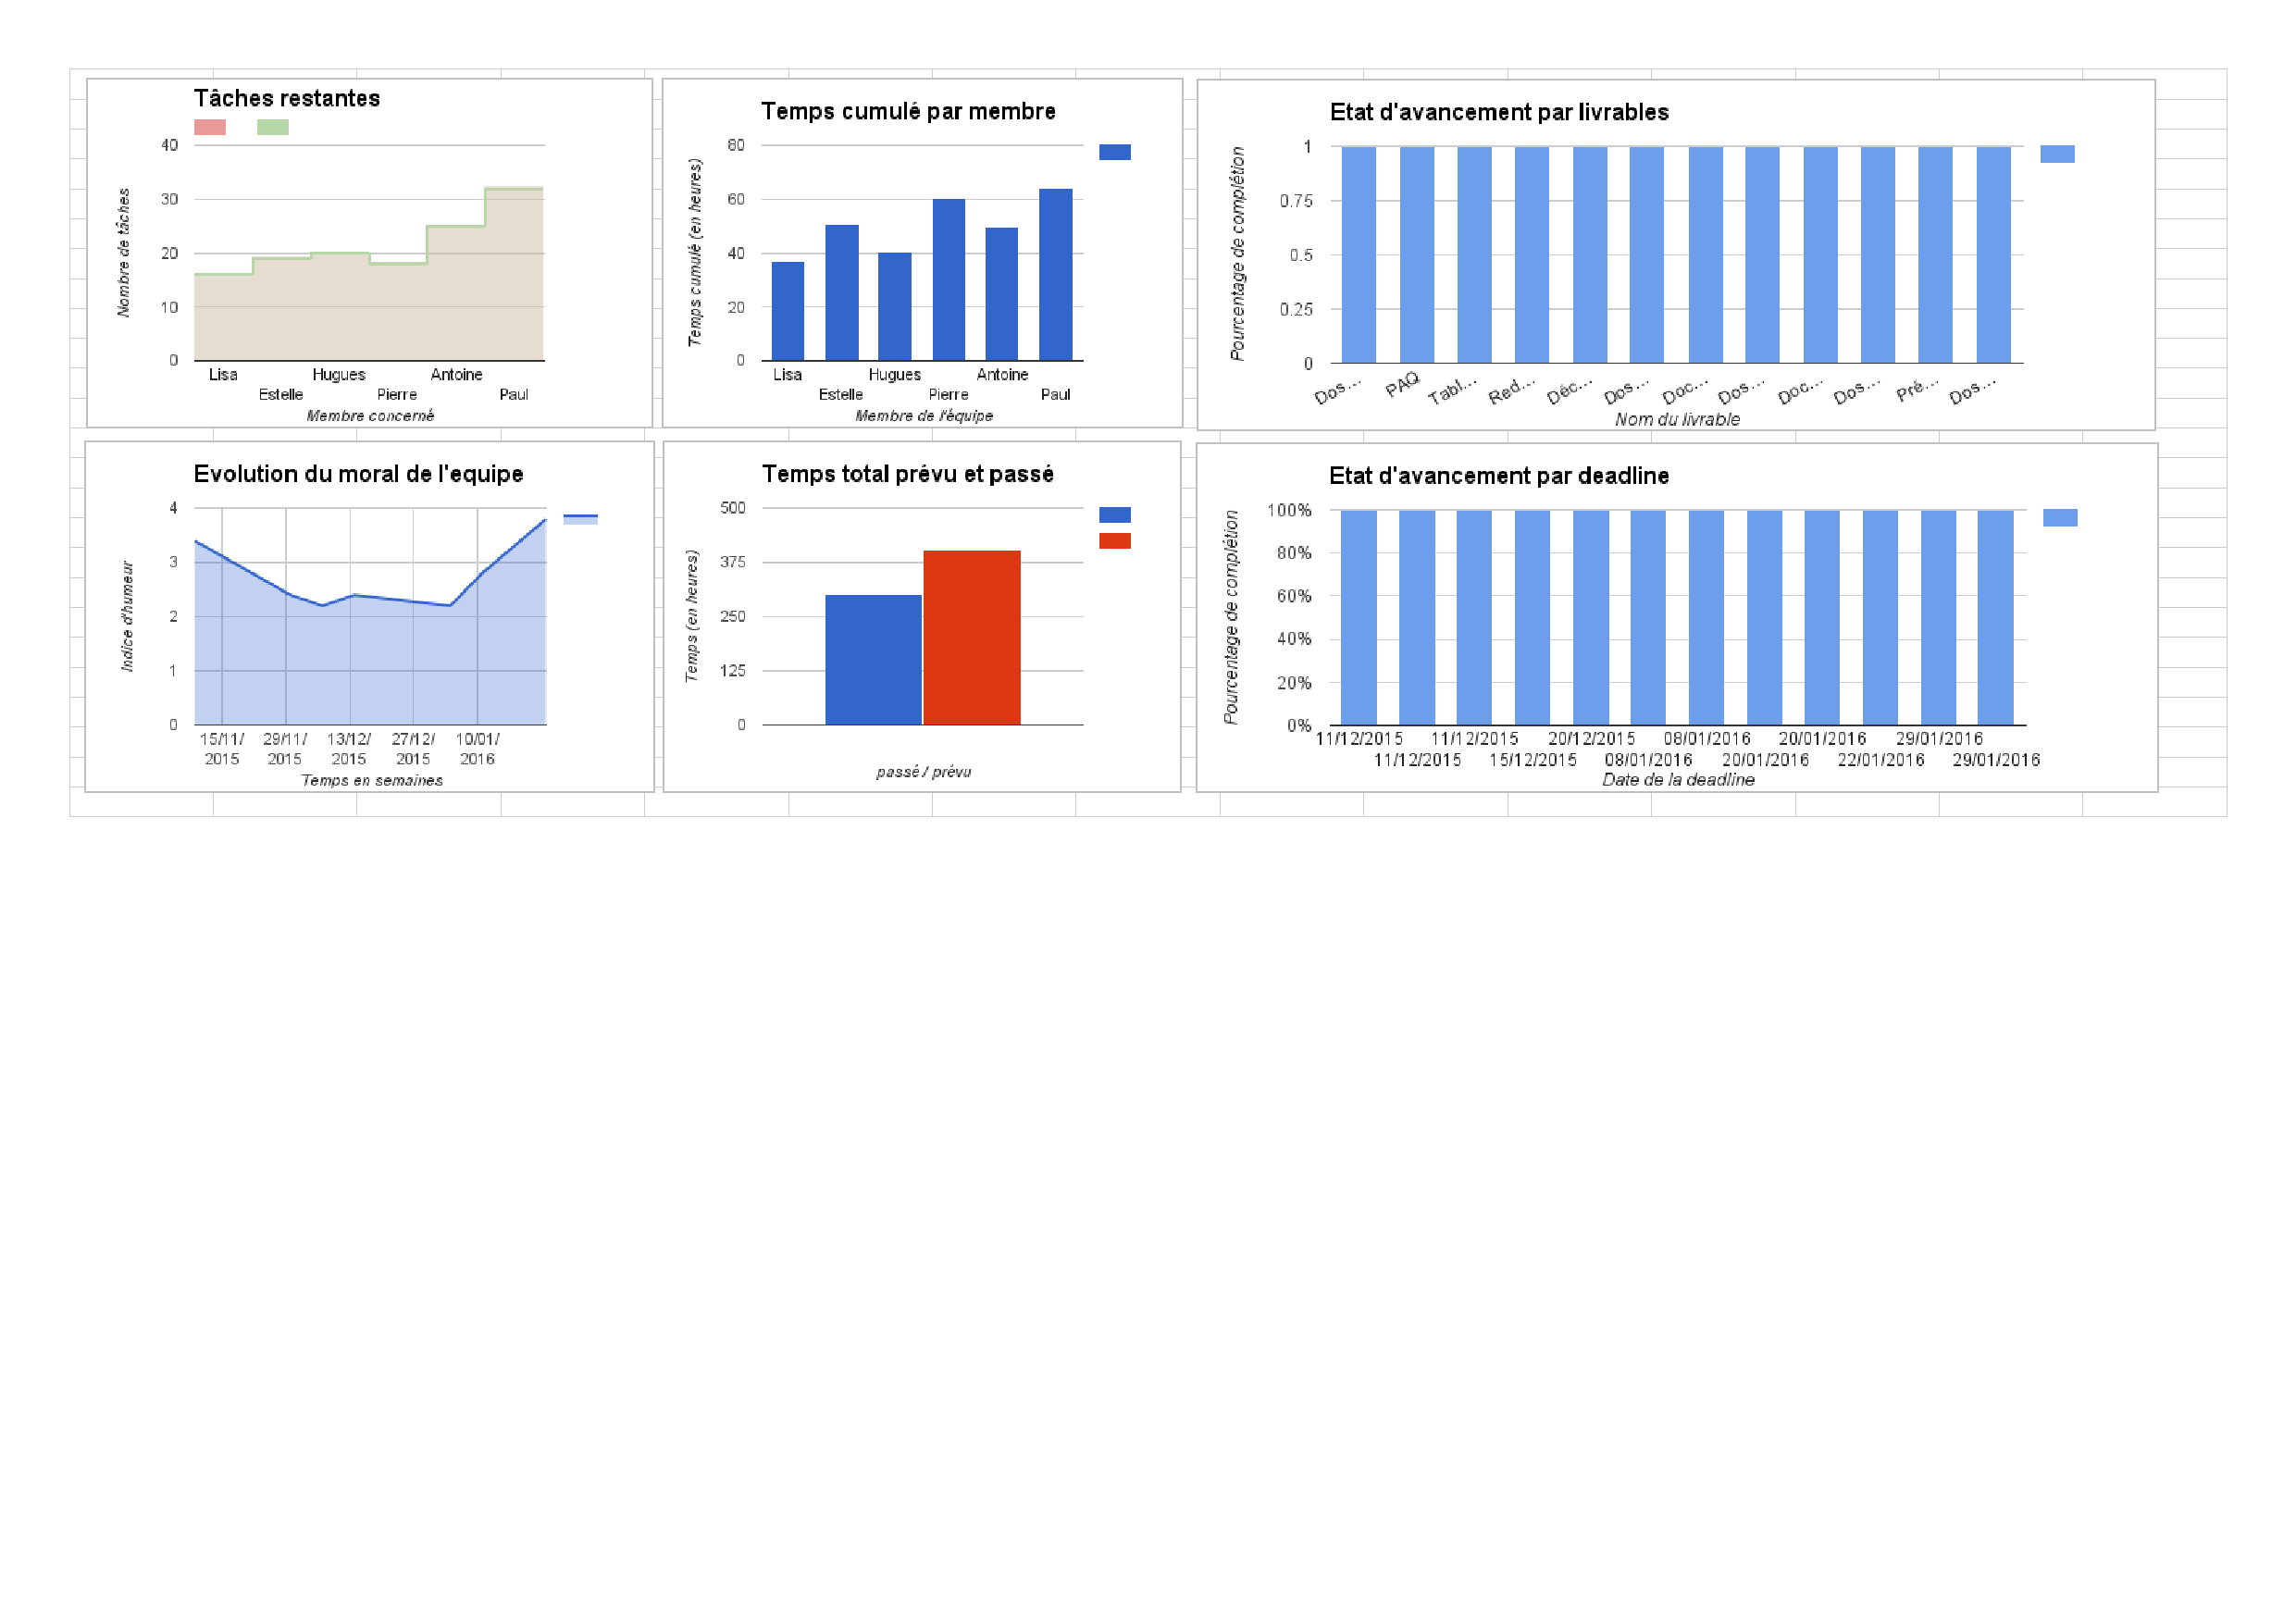
\includepdf[pages=-]{tdb/TdB.pdf}


%% Inclure une figure :
%\begin{figure}[H]
%    \label{fig-LABEL-DE-LA-FIGURE}
%    \noindent\makebox[\textwidth]{\includegraphics[width=10cm]{figures/NOM-DE-LA-FIGURE.png}}
%    \caption{TEXTE DE LA LEGENDE}
%\end{figure}

%%% End document
\end{document}
